\documentclass[twocolumn,aps,tightenlines,floatfix,showpacs]{revtex4}
\usepackage{graphicx,mathtools}
\begin{document}

\title{First principles calculations for coefficients of the isobaric
mass multiplet equation in the fp shell}


\author{W.~E.~Ormand}
\affiliation{Lawrence Livermore National Laboratory, Livermore, CA 94551, USA}
\author{B.~A.~Brown} 
\affiliation{Department of Physics and Astronomy and National Superconducting Cyclotron Laboratory,
Michigan State University, East Lansing, MI 48824-1321, USA}
\author{M.~Hjorth-Jensen}
\affiliation{Department of Physics and Astronomy and National Superconducting Cyclotron Laboratory,
Michigan State University, East Lansing, MI 48824-1321, USA}
\affiliation{Department of Physics, University of Oslo, N-0316, Oslo, Norway}

\begin{abstract}
We present the first calculations for the coefficients of the isobaric
mass multiplet equation (IMME)
for nuclei from $A=42$ to $A=54$ based input from various nucleon-nucleon interactions.
We show that there is clear dependence on the short-ranged charge-symmetry
breaking (CSB) part of the strong interaction. There is a significant
variation in the CSB part between the commonly
used CD-Bonn, N$^3$LO and Argonne V18 nucleon-nucleon
interactions. All of them give a CSB contribution that is too large
compared to experiment.
\end{abstract}

\pacs{}


\maketitle


Charge symmetry breaking in nuclear systems is due to the difference between the masses of up and down 
quarks, reflected in slightly differing masses between neutrons and protons \cite{miller2006}. 
This leads to the assumption of the near 
charge symmetry and isospin symmetry independence of nuclear forces.
When electromagnetic effects are taken out, observables like bulk properties and excited states 
should be nearly charge independent. In order to more text will be added...



We have performed a series of shell-model calculations using the
program BIGSTICK to compute the $c$-coefficients of the IMME for
$1p0f$-shell nuclei with $ 42 \le $ A $ \le 54$. The pertinent
effective interactions for the degrees of freedom of the $1p0f$ shell
were derived using many-body perturbation theory, see for example
Ref.~\cite{mhj1995}. The two-body matrix elements where computed in
two steps, first by renormalizing the nuclear two-body interactions
using both a $G$-matrix approach and the so-called V$_{lowk}$
method. As models for the nuclear interactions, we employed the
N$^3$LO \cite{entem2003}, the AV18 \cite{argonne1995} and the CD-Bonn
\cite{cdbonn2001} interaction models. These interaction models allow
for a breaking of isospin symmetry and charge symmetry and include the
isotensor and isovector components of the strong interaction.  The
renormalized nucleon-nucleon interactions were computed using a
harmonic oscillator basis with an oscillator energy $\hbar\omega
=10.5$ MeV with an effective Hilbert space defined the twelve first
oscillator shells. The V$_{lowk}$ interactions were obtained with a
cut-off parameter of $\Lambda$ = 2.1 fm$^{-1}$.  For the N$^3$LO and
the CD-Bonn interactions, the Coulomb interaction was added after the
renormalization process.  The second step consisted in obtaining an
effective interaction tailored to a small shell-model space. This was
achieved using many-body perturbation theory up to third-order in the
renormalized nucleon-nucleon interactions, including so-called folded
diagrams \cite{mhj1995}. All codes used to generate these interactions
are available online, see Ref.~\cite{mhjgit}.  The renormalization was
performed with and without the Coulomb interaction, and the Coulomb
two-body matrix elements were obtained from the difference between
these proton-proton ($pp$) matrix elements. The renormalized
interaction computed without Coulomb was then decomposed into the
three isospin components: isoscalar (rank 0), isovector (rank 1), and
isotensor (rank 2), defined in terms of the $T=1$ components of the
$pp $, neutron-neutron ($nn$) and proton-neutron ($pn$) interactions
via
\[
v^{(0)}  =  \frac{1}{3} \left(v_{pp} + v_{nn} + v_{pn}\right),
\]
\[
v^{(1)}  =  v_{pp} - v_{nn},
\]
and
\[
v^{(2)}  =  v_{pn} - \frac{1}{2}(v_{pp} + v_{nn}).
\]

The $c$-coefficients of the IMME were obtained utilizing first-order
perturbation theory. The base for each calculation was the eigenstate,
$E_{0}$ for each member of the $T=1$ triplet, $ \vert T_{z} \rangle$,
obtained using the isoscalar GX1A Hamiltonian. The GX1A interaction
was used instead of the $v^{(0)}$ interaction obtained from the
realistic interaction described above because of well-known extensions
that must be included to properly capture the behavior of higher-order
components and the three-body interaction in the traditional
configuration-interaction shell model for atomic nuclei. The
expectation value of the Coulomb, isovector, and isotensor
interactions are then computed to give the full energy for each state,
\[
E(T_{z}) = E_{0} + \langle T_{z} \vert   v^{{\rm Coul}} + v^{(1)} + v^{(2)}\vert T_{z} \rangle
\]
and the c-coefficient is then
\[
c = [E(T_{z} =1) - 2E(T_{z} =0) + E(T_{z} =-1)]/2.
\]
The $A$-dependence was properly accounted for by scaling the Coulomb
component by $  \sqrt{\hbar\Omega(A)/10.5}  $, while the isovector and
isotensor interactions were assumed to have the same A-dependence as
the GX1A interaction. For each $A$-value, $\hbar\Omega(A)$ was
determined by reproducing the rms radius obtained from a Hartee-Fock
calculation using the SKX Skyrme interaction.

Figure 1 shows the results CD-Bonn in first, second and third order.
The contributions are divided into Coulomb (full lines)
and CSB (dashed lines). The $J$-dependence of these
two contribution is very different. The long-range Coulomb
has a relatively flat $J$-dependence with only
a small rise at $J=0$. The CSB contribution at $A=42$
shows a peak at $J=0$ with a sharp drop towards $J=2$
that is characteristic of a short-ranged interaction.
for $A=42$ $J=6$ is the maximum
spin (for $T=1$) in the $1p0f$ model space.
For higher A values this sharp drop at $  J=2  $ is replaced
by a linear drop to $J=6$ due to configuration mixing.
CSB is very small for $J=8$ and $10$.
The experimental data is from the compilation \cite{2013la}. 
For A=46 we use the results from Fig.~2 of \cite{2001ga}.

Both Coulomb and CSB have a small increase at $  J=12  $.
The reason for this is that
protons with $  J=6  $ and neutrons with $  J=6  $
are maximally aligned results in an enhancement of the
overlapping proton and neutron density distributions.

\begin{figure}
%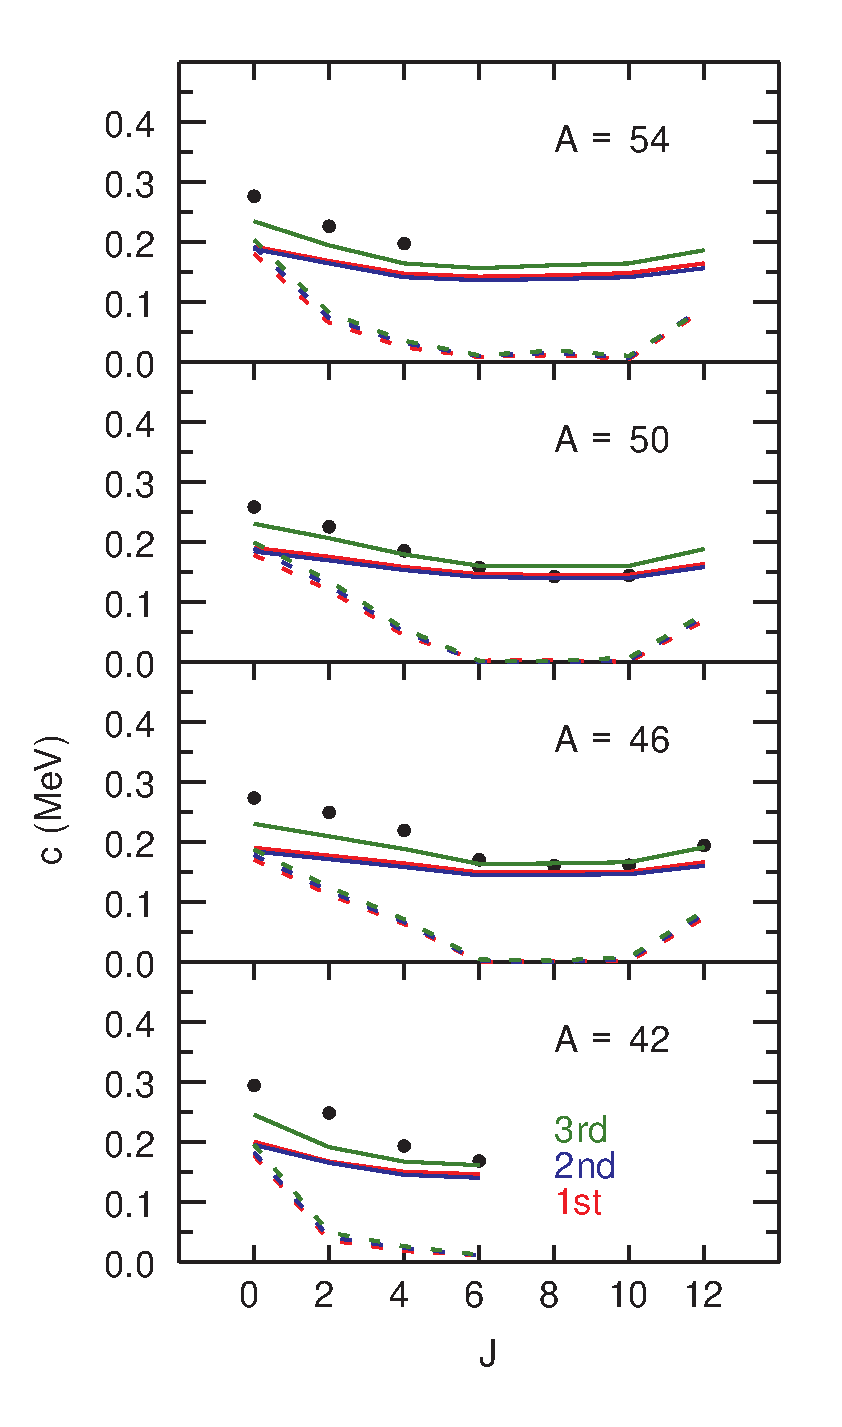
\includegraphics[scale=0.35]{ccd.eps}
\caption{(color online) Results for the CD-Bonn potential
in 1st, up to 2nd and up to 3rd order.
The black circles
are the experimental data. The solid lines show the Coulomb
contribution, and the dashed lines show the CSB contribution.}
\end{figure}
\begin{figure}
%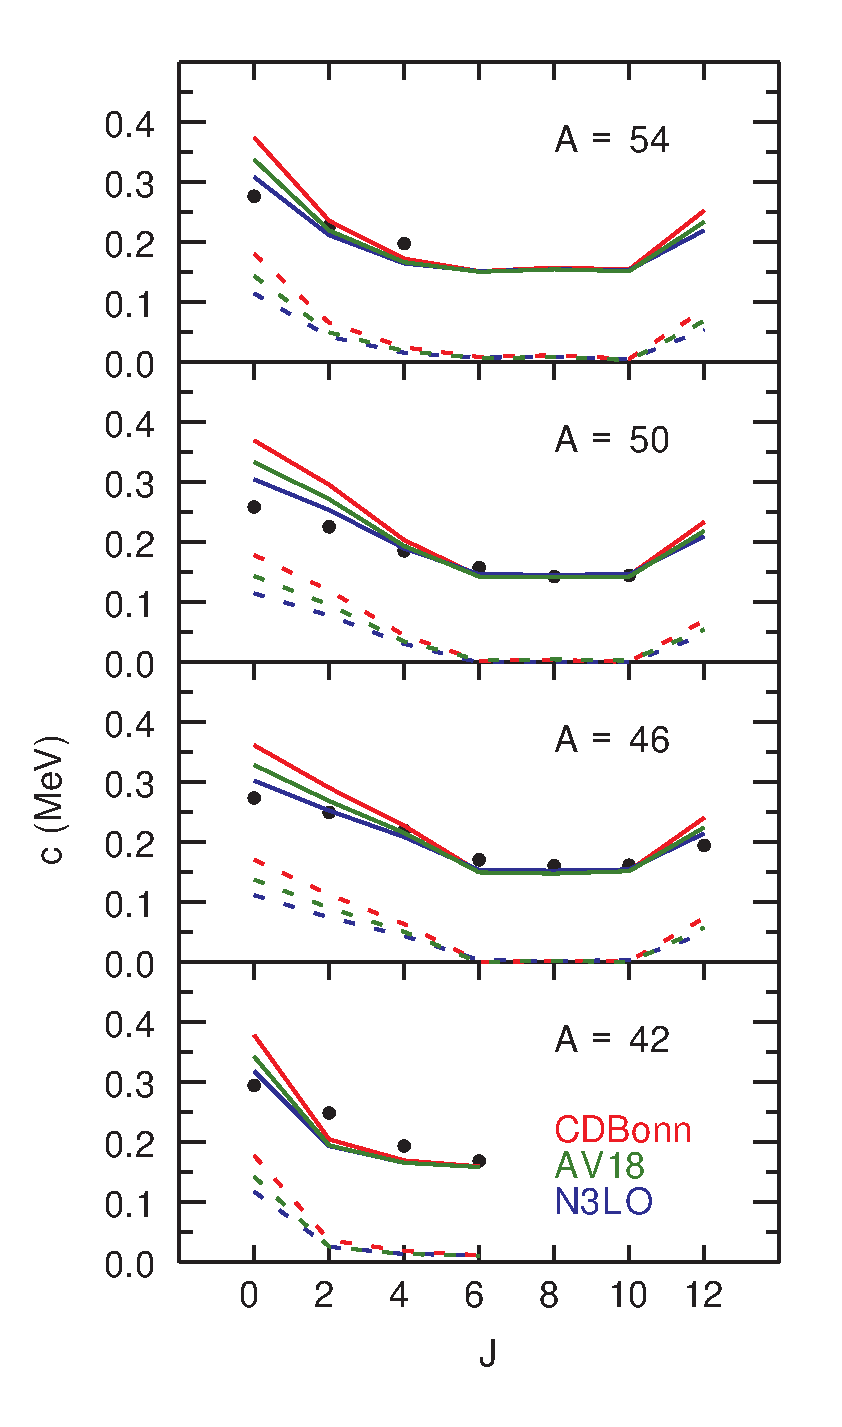
\includegraphics[scale=0.35]{c1.eps}
\caption{(color online) 1st order calculations compared to
experiment. The black circles
are the experimental data. The solid lines show the sum of Coulomb and
CSB
contributions. The dashed lines show only the CSB contribution.}
\end{figure}
\begin{figure}
%\includegraphics[scale=0.35]{c3.eps}
\caption{(color online) Calculations up to 3rd order compared to
experiment. See caption to Fig 2.}
\end{figure}
\begin{figure}
%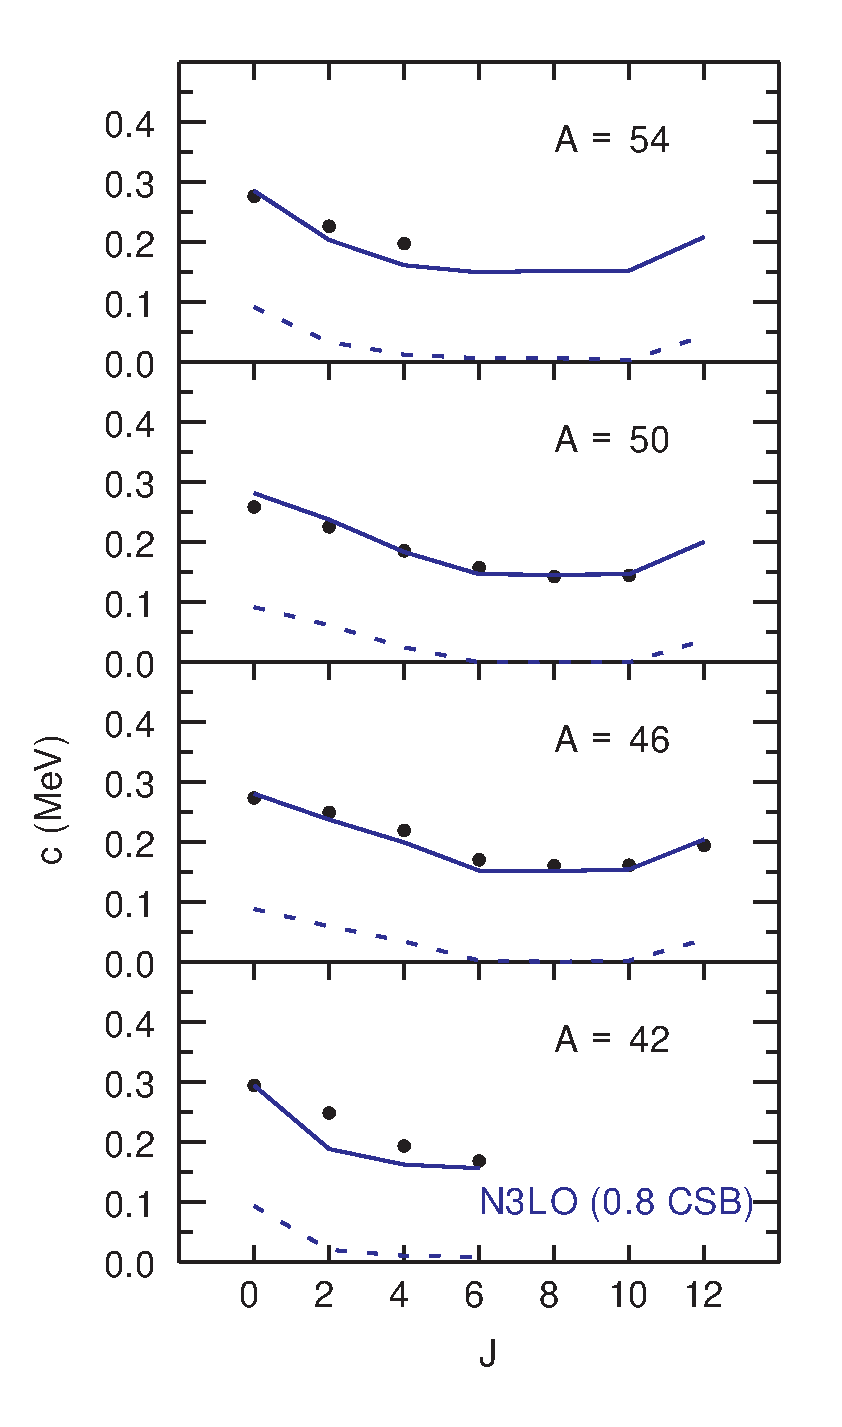
\includegraphics[scale=0.35]{c1e.eps}
\caption{(color online) 1st order calculations for N$^3$LO
with the CSB part multiplied by 0.8 and compared to
experiment. See caption to Fig 2.}
\end{figure}



The CSB contribution turns out to be
almost order independent.
The Coulomb contribution is almost the same in 1st and 2nd order
but increases 10-20\% in 3rd order. It is remarkable that the
experimental data are in rather good agreement with the 3rd order
Coulomb result. There does not seem to be a need for CSB
even though this component is
known to be important in the NN scattering data that is
incorporated into the potential models.

Figure 2 shows the results for the three potential models in 1st order.
This shows that the CSB contribution is model dependent.
There could be two reasons for this. The NN potential
inputs for CSB are different.
Or if they are the same the short range correlation effects
taken into account in the V$_{lowk}$ renormalization are
different. The results with N$^3$LO is in best agreement with experiment.

Figure 3 shows the results for the three potentials in 3rd order.

Our work guides future investigations in directions.
For better first principles calculations, one should
understand the origin of the
different CSB contributions from three potentials.
In particular in the spirit of using nuclear data to
constrain the NN and NNN potentials (in addition to NN scattering
data) one should use the c-coefficient as a constraint on the
CSB part. From a practical point of view we start with the
fact that 1st order Coulomb plus CSB is already close to the data.
We can make it almost perfect by taking 1st order Coulomb
and adding 80\% of the N$^3$LO CSB part. This is shown in Fig.~4.
The largest deviation from experiment comes for $  J=2  $ at A=42.
However, $  A=42  $ is just at the beginning of the $  1p-0f  $
model space and it is well know that admixtures from
core excitations from the
$  0s-1d  $ shell are very important especially for $  J=0  $ and $  J=2  $.
For example, the 2$^{ + }$ to 0$^{ + }$ B(E2) value for $^{42}$Ca is about 10 times
larger in experiment than compared to theory. The experimental
fall off from $  J=0  $ to $  J=6  $ in A=42 looks like calculation
for A=46. The theoretical wavefunctions for
A=42 are dominated by $  (f_{7/2})^{2}  $ configurations
and the wavefunctions for $  A=54  $ are dominated by
$  (f_{7/2})^{-2}  $ configurations. These two configuration
have the same spectra (except for a small mass dependence).
Compared to $  A=42  $ the
$  J  $ dependence observed for $  A=54  $ is closer that
expected for a these pure configurations.






BAB acknowledges U.S. NSF Grant No. PHY-1404442.
MHJ acknowledges U.S. NSF Grant No. PHY-1404159 and  the Research Council of
Norway under contract ISP-Fysikk/216699.

\begin{thebibliography}{99}
\bibitem{miller2006} G.~A.~Miller, A.~K.~Opper, and E.~J.~Stephenson, Annu.~Rev.~Nucl.~Sci.~{\bf 56}, 253 (2006).
\bibitem{2013la} Y.~H.~Lam, B.~Blank, N.~A.~Smirnova, J.~B.~Bueb, and M.~S.~Antony, At.~Data and Nucl.~Data Tables {\bf 90}, 680 (2013). 
\bibitem{2001ga} P.~E.~Garrett {\em et al.}, Phys.~Rev.~Lett.~{\bf 87}, 132502 (2001). 
\bibitem{mhj1995} M.~Hjorth-Jensen, E.~Osnes, and T.~.T.~.S.~Kuo, Phys.~Rep.~{\bf 261}, 125 (1995).
\bibitem{entem2003} D.~R.~Entem and R.~Machleidt, Phys.~Rev.~C {\bf 68}, 041001(R) (2003).
\bibitem{argonne1995} R.~B.~Wiringa, V.~G.~J.~Stoks, and R.~Schiavilla, Phys.~Rev.~C {\bf 51}, 38 (1995).
\bibitem{cdbonn2001} R.~Machleidt, Phys.~Rev.~C {\bf 63}, 024001 (2001).
\bibitem{mhjgit} All codes used to generate the effective interactions are available at \url{ https://github.com/ManyBodyPhysics/CENS}.
\end{thebibliography}

\end{document}

\cite{Heyde2011} K. Heyde and J.L. Wood, Revs. Mod. Phys. {\bf 83}, 1467
(2011).

